\chapter{Anhang}


\section{Quellcodeauszug}
Im der Abbildung \ref{aircraftFamilySelectionViewModelClass} ist das vollständige ViewModel für die Auswahl des Flugzeugprogramms zu sehen. Die Klasse wurde für ein Beispiel der Navigation in der Anwendung verwendet und ist im Text referenziert.

\begin{lstlisting}[caption=Vollständige SelectAircraftFamilyViewModel Klasse für die Flugzeugprogrammauswahl]
/// <summary>
    /// This View Model has the logic for aircraft family selection. Normally its the first view if
    /// a new configuration is started.
    /// </summary>
    public class SelectAircraftFamilyViewModel : GridHolderViewModel
    {
        private AircraftModel _model;
        private ICommand _familySelectedCommand;

        public SelectAircraftFamilyViewModel()
        {
            Headline = "select aircraft family";
            _model = new AircraftModel();
            InitializeDataSource();
        }

        private void InitializeDataSource()
        {

            DataGroupElements = new ObservableCollection<IIdentable>
                {
                    new AircraftProgrammGroup(_model.GetAllAircraftProgramms())
                }; 
        }

        public ICommand SelectAircraftCommand
        {
            get { return _familySelectedCommand ?? (_familySelectedCommand = new RelayCommand<DataCommon>(SaveSelectionAndNavigateToSummaryPage)); }
            set
            {
                _familySelectedCommand = value;
                OnPropertyChanged();
            }
        }

        private void SaveSelectionAndNavigateToSummaryPage(DataCommon data)
        {
            var selectedProgramm = GetSelectedProgramm(data.UniqueId);
            _model.SelectAircraftProgramm(selectedProgramm);
            var classToNavigate = SimpleIoc.Default.GetInstance<ISummary>();
            var navigationService = SimpleIoc.Default.GetInstance<INavigationService>();
            navigationService.Navigate(classToNavigate.GetType());
        }

        private AircraftProgramm GetSelectedProgramm(string uniqueId)
        {
            return _model.GetAllAircraftProgramms().FirstOrDefault(programm => programm.UniqueId.Equals(uniqueId));
        }

        public override void Initialize(object parameter)
        {
            
        }
\end{lstlisting} 
\label{aircraftFamilySelectionViewModelClass}

 
\section{Evaluationsbögen} \label{anhangEva}
Die Fragebögen für die Experten und die Benutzer sind auf den folgenden beiden Seiten angehängt.

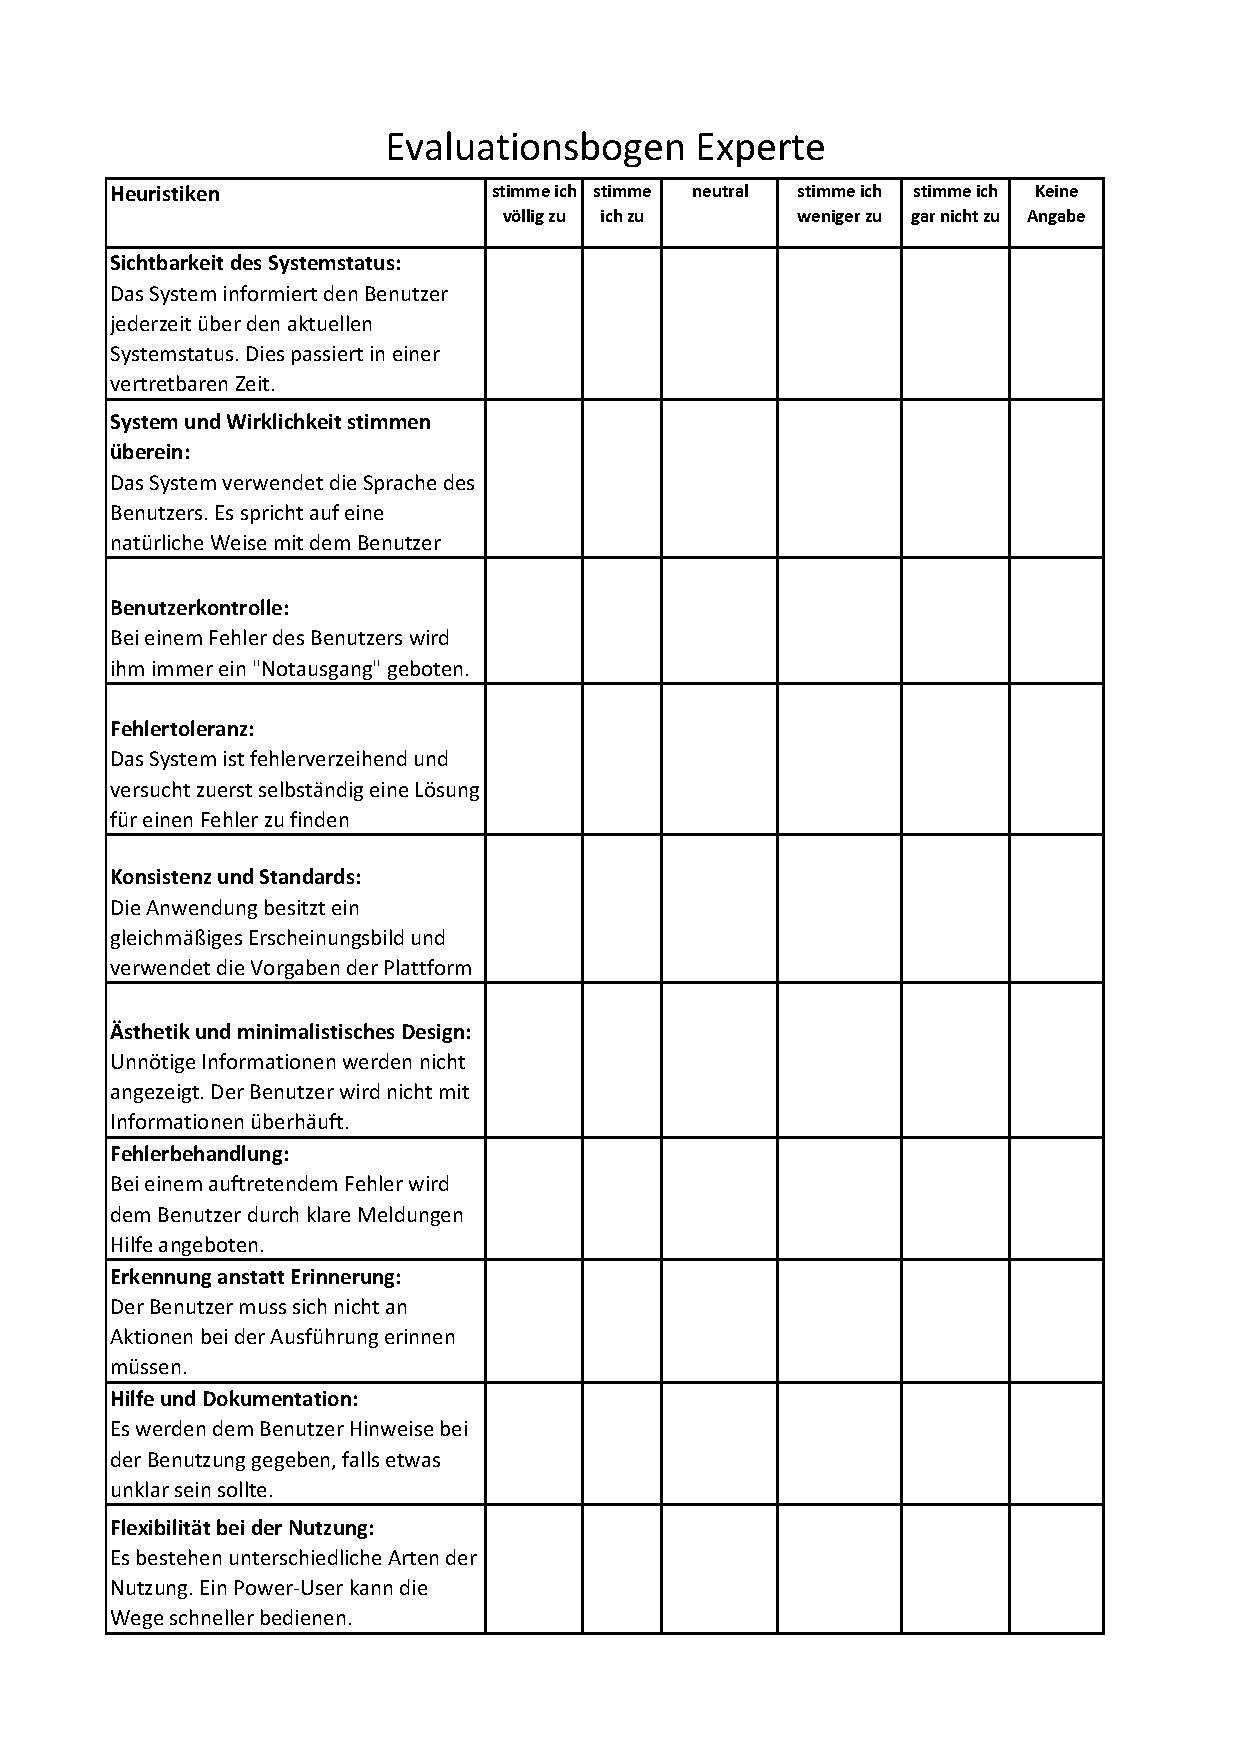
\includepdf[pages=1]{anhang/evaluationsbogenExperte.pdf}
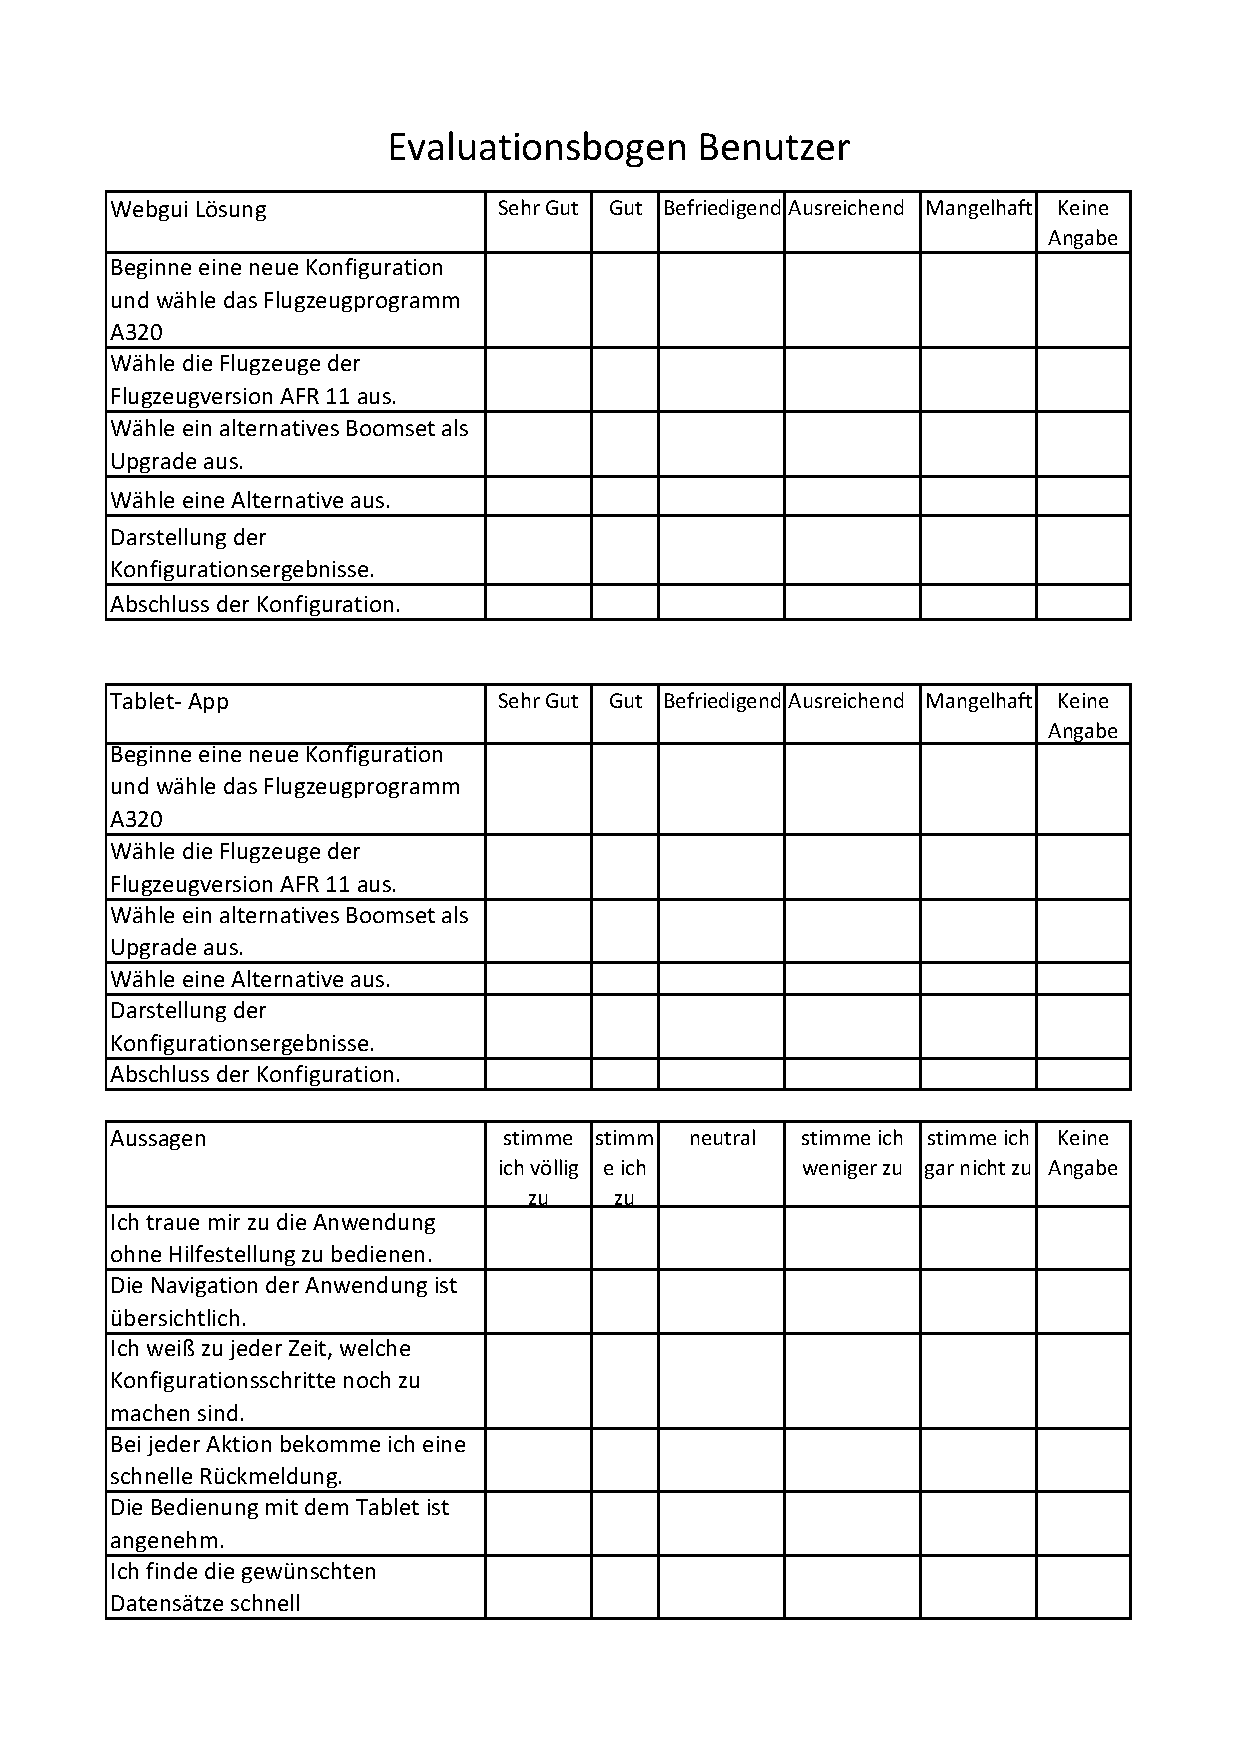
\includepdf[pages=1-2]{anhang/evaluationsbogenUser.pdf}

\section{Zusätzliche Evaluationsergebnisse} \label{anhangEvaErg}
Im Folgenden wird das Ergebnis des ersten Teils vom Benutzerfragebogen dargestellt. In Abbildung \ref{bewertungWebguiComplete} ist die vollständige Auswertung der Fragebögen für die Fragen zur vorhandenen Konfigurationslösung zu sehen. Da beide Anwendungen unterschiedliche Zielgruppen und Ziele verfolgen, wurde kein Vergleich durchgeführt. Die Fragen waren für die Darstellung der Unterschiede, sowie für das Durchführen der gemeinsamen Aktionen hilfreich. \par 
\begin{figure}[H]
\centering
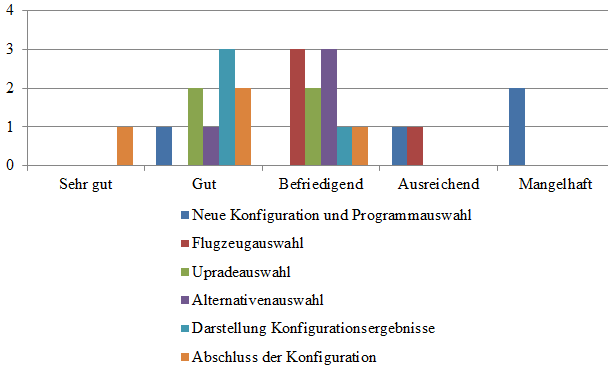
\includegraphics{images/bewertung_webgui}
\caption{Ergebnis der Fragen zur vorhandenen Konfigurationslösung}
\label{bewertungWebguiComplete}
\end{figure}
